
\section{Objectives}

Monitoring fish stocks is a critical component of sustainable fisheries management in the Southern Gulf of St. Lawrence.
One key aspect of this work is understanding the population dynamics of various fish stocks, which involves accurate age determination.
Age data are essential for modeling growth patterns, understanding reproduction, and assessing the health and sustainability of fish populations.

\subsection{Goal of the analysis}

The primary objective of this project is to develop and implement a machine learning-based predictive model capable of estimating the age of fish from otolith images.
This model will automate the process of age determination, reduce the potential for human error, and provide quicker assessments for large datasets.

Specifically, the objectives of the project include:

\begin{itemize}
    \item Data Collection and Preparation: Compile an archive of otolith images along with corresponding fish age, length, and weight data.
    \item Model Development: Create a predictive model using machine learning techniques to automatically identify annuli in otolith images and predict the age of the fish.
    \item Model Validation: Validate the model's accuracy using a separate set of otolith images and corresponding age data.
\end{itemize}

The training dataset will consist of fish otolith images originating from two Atlantic Canadian species of economic and ecological importance:
American plaice (\textit{Hippoglossoides platessoides}) and Atlantic herring (\textit{Clupea harengus}).


\subsection{Rationale behind the analysis}

Fish age is commonly determined by examining biological materials such as otoliths (inner ear bones) and scales.
These materials exhibit growth rings, or \enquote{annuli} (Figure~\ref{fig:plaice_oto_example} and Figure~\ref{fig:herring_oto_example}), which can be counted similarly to tree rings.
Each ring represents a period of growth, typically corresponding to one year in the life of the fish.
However, manually counting these rings can be time-consuming, subjective, and prone to human error.
Organizations that age fish are typically limited by the amount of time it takes the team of human experts to read the otolith samples.

The development of an automated system for predicting fish age based on otolith images would significantly improve the accuracy and speed of age estimation.
At a minimum, having a machine learning (ML) model to complement the work of human agers will provide an aspect of quality control to the aging process.
At best, these models might actually help speed up the processing time required for aging fish.

\pagebreak

\begin{figure}
    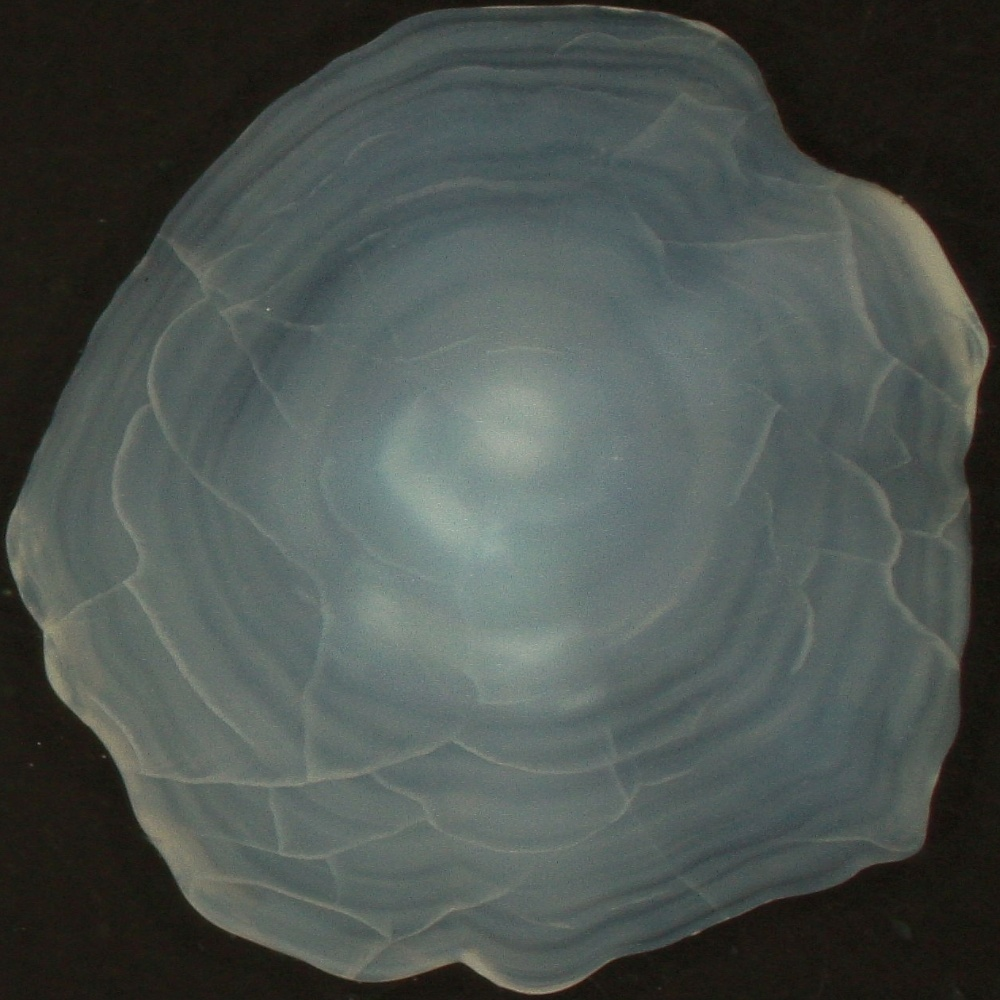
\includegraphics[width=\linewidth]{plaice_otolith_example}
    \caption{An example of an otolith image taken from an American Plaice.}
    \label{fig:plaice_oto_example}
\end{figure}

\begin{figure}
    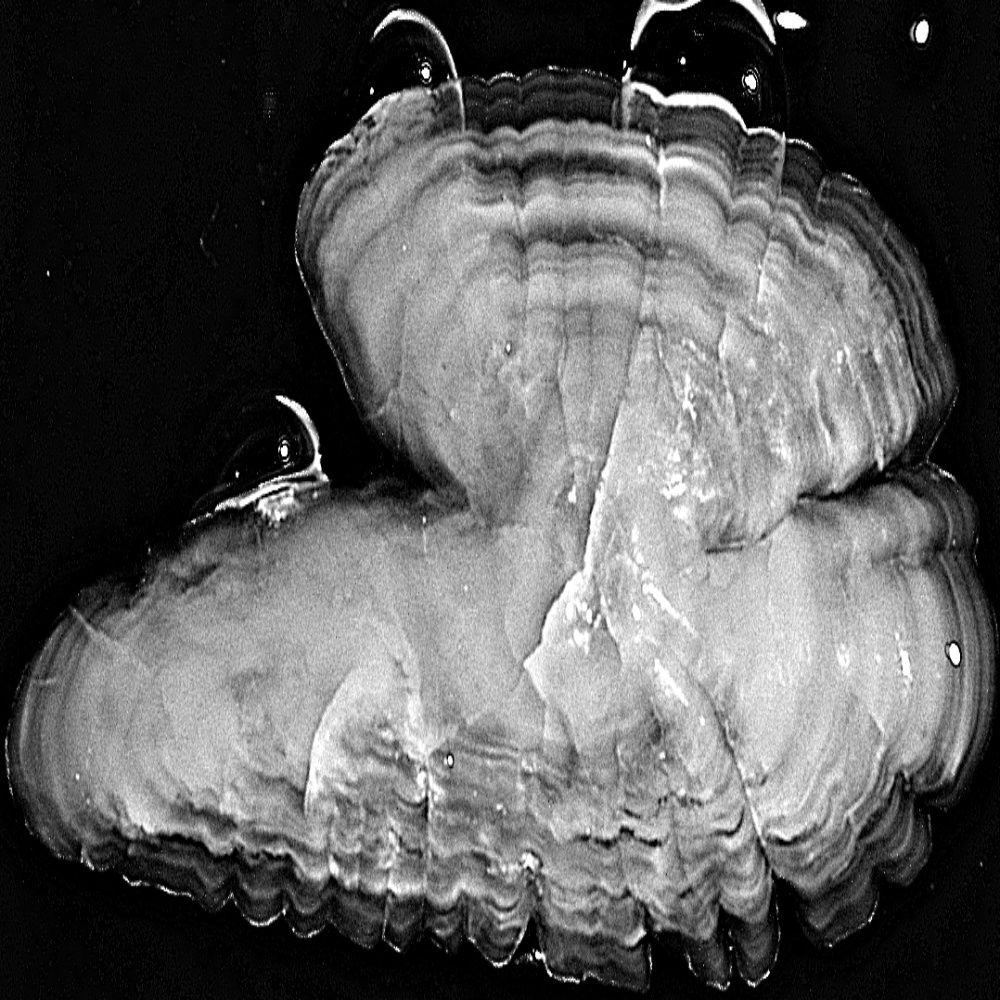
\includegraphics[width=\linewidth]{herring_otolith_example}
    \caption{An example of an otolith image taken from an Atlantic Herring.}
    \label{fig:herring_oto_example}
\end{figure}

